\section{\JVT sample dependence}
\label{app:sample_dep}


We study the dependence of JVT
We test the potential sample dependence of \JVT by deriving the \JVT likelihood in \Figref{fig:JVTLikelihood} using a sample of $\Zboson \to \mu\mu$ events and 
evaluating its performance in QCD dijet and $\Zboson \to \mu\mu$ events. The resulting four efficiency \vs fake rate curves are shown in \Figref{fig:SampleDependence}. No
significant sample dependence is observed, 
% suggesting that the level of separation between hard-scatter and pileup jets does not significantly degrade when the \JVT likelihood is derived from a sample with slightly different flavor composition. 
suggesting that the \JVT likelihood in \Figref{fig:JVTLikelihood} does not underperform when applying it to different physics processes. 
The difference in the fake rate \vs efficiency curves between \Figref{fig:SampleDependence_dijets} and \Figref{fig:SampleDependence_Zmumu} is attributed to the 
different flavor composition of the jets in QCD dijet and $\Zboson \to \mu\mu$ events. 
%--------------------------
\begin{figure}[!htbp]
  \centering
  \subfigure[]{
  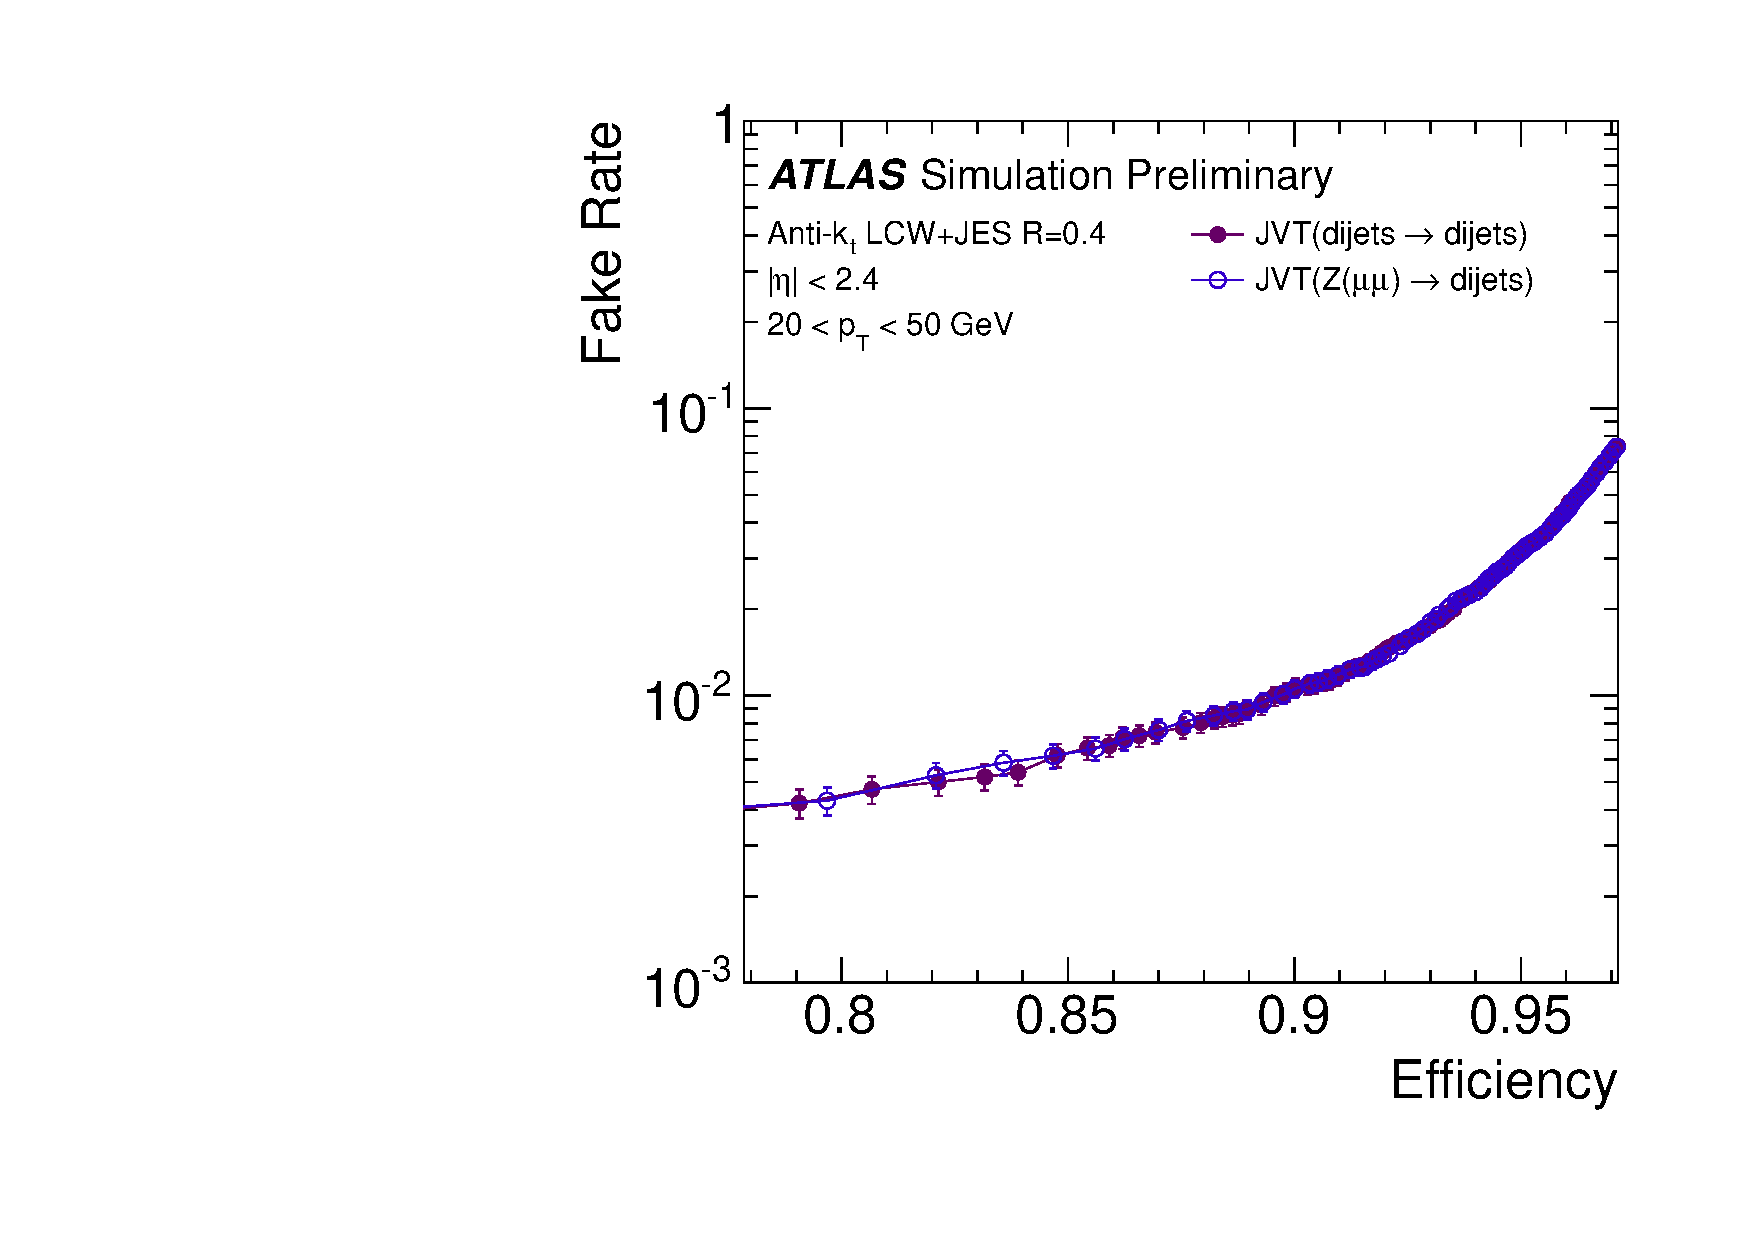
\includegraphics[width= 0.48\textwidth]{ROC_pt20to50_JVTdijet_JVTZmumu_appliedToDijets}
  \label{fig:SampleDependence_dijets}
  }
  \subfigure[]{
  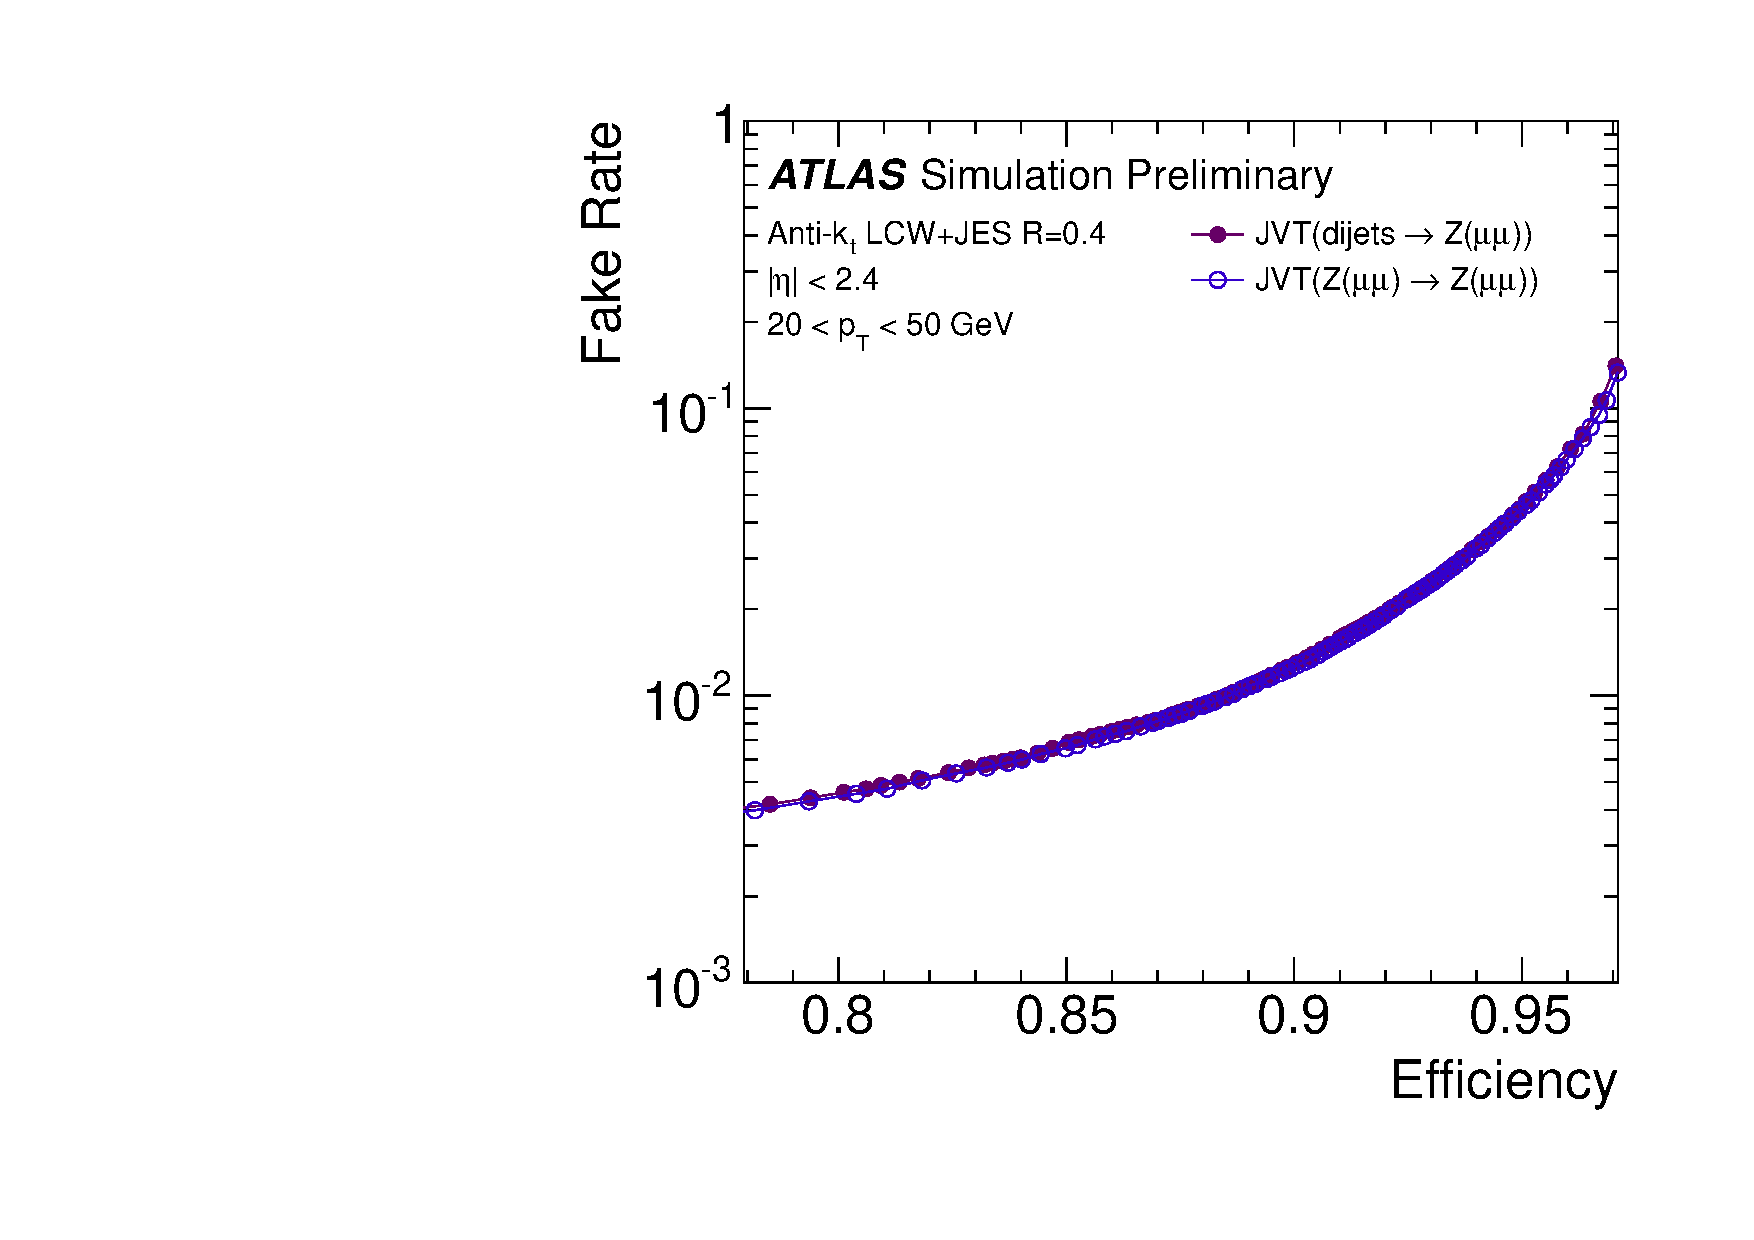
\includegraphics[width=0.48\textwidth]{ROC_pt20to50_JVTdijet_JVTZmumu_appliedToZmumu}
  \label{fig:SampleDependence_Zmumu}
  }
  \caption{Efficiency \vs fake rate curve for JVT evaluated on $20 < \pT < 50\GeV$ jets from a sample of QCD dijet events (a) and $\Zboson \to \mu\mu$ events (b). 
           The curve represented by solid magenta markers are obtained when deriving the \JVT likelihood on a QCD dijet sample. For the 
           open blue markers, the \JVT likelihood was derived from $\Zboson \to \mu\mu$ events. No significant sample dependence is observed. }
\label{fig:SampleDependence}
\end{figure}
%------------------------
